
\section{File Conversion}

    \subsection{Building}

        Special configurations were set in order to build the project.  There were three places where the configuration was set.  To access the configurations, right click on the \texttt{FileConversion} line, below the \texttt{Solution} line, above all of the source files, and click \texttt{Properties}.  
        
        \begin{enumerate}
            \item Open the \texttt{C/C++} drop-down, select General.  Click on the first line, \texttt{Additional Include Directories}, select the down arrow at the end of the line, and select \texttt{<Edit...>}.  The two configurations are shown in Figure \ref{fig:fileconversionVSConfig1}.  These are the include directories for the libraries.   

            \begin{figure}[H]
                \includegraphics[width=\textwidth]{Deployment/FileConversionVSConfig1}
                \centering
                \caption{File Conversion VS Configuration Include Directories}
                \label{fig:fileconversionVSConfig1}
            \end{figure}

            \item Under the Linker drop-down in the Properties, select General.  Edit the contents of the line labeled \texttt{Additional Library Directories} by clicking on the line, clicking the down arrow at the end of the line, and selecting edit.  The contents of this field are shown in Figure \ref{fig:fileconversionVSConfig2}.  This points the linker to the flies needed for the libraries.

            \begin{figure}[H]
                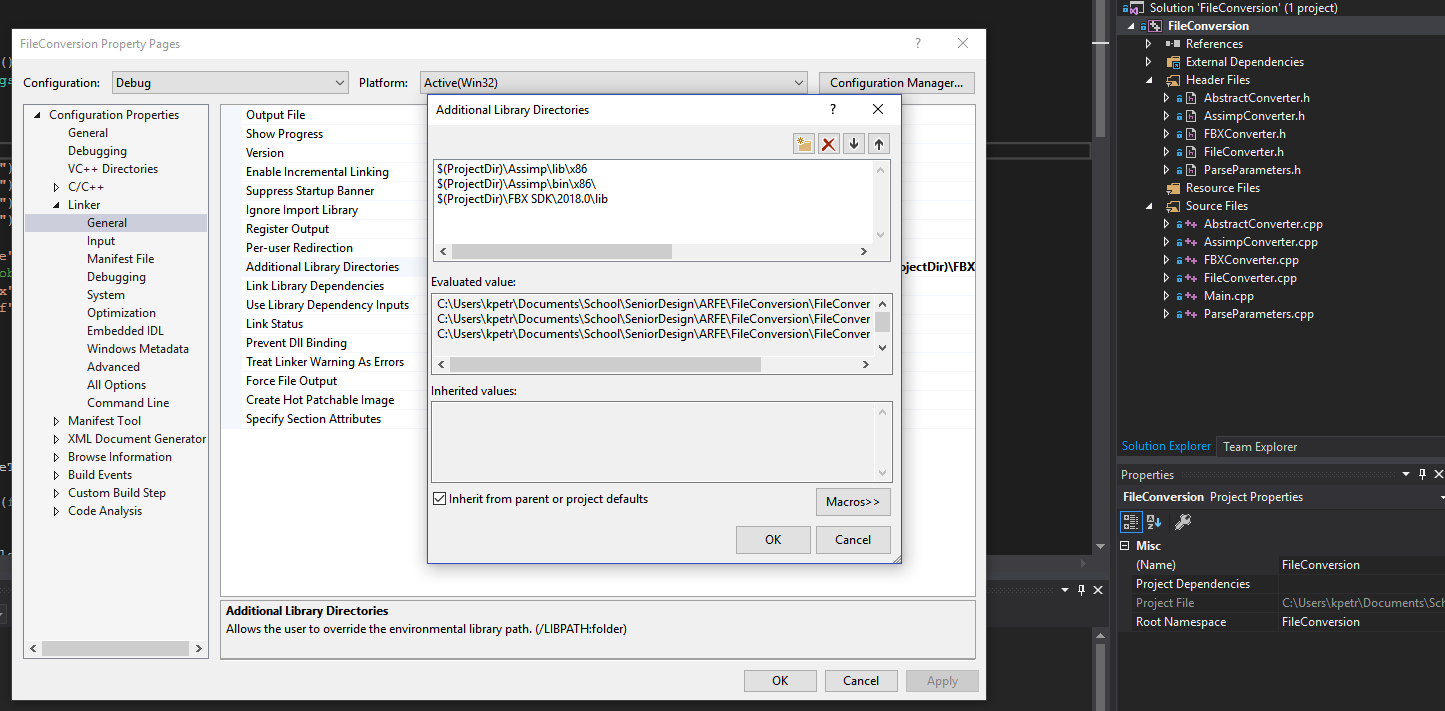
\includegraphics[width=\textwidth]{Deployment/fileConversionVSConfig_Linker}
                \centering
                \caption{File Conversion VS Configuration Linker Configuration - General}
                \label{fig:fileconversionVSConfig2}
            \end{figure}

            \item Under the Linker drop-down in the Properties, select \texttt{Input}.  Edit the content of the first line (labeled \texttt{Additional Dependencies}) by selecting the line, clicking on the down arrow, and clicking edit.  The configuration for this section can be found in Figure \ref{fig:fileconversionVSConfig2}.

            \begin{figure}[H]
                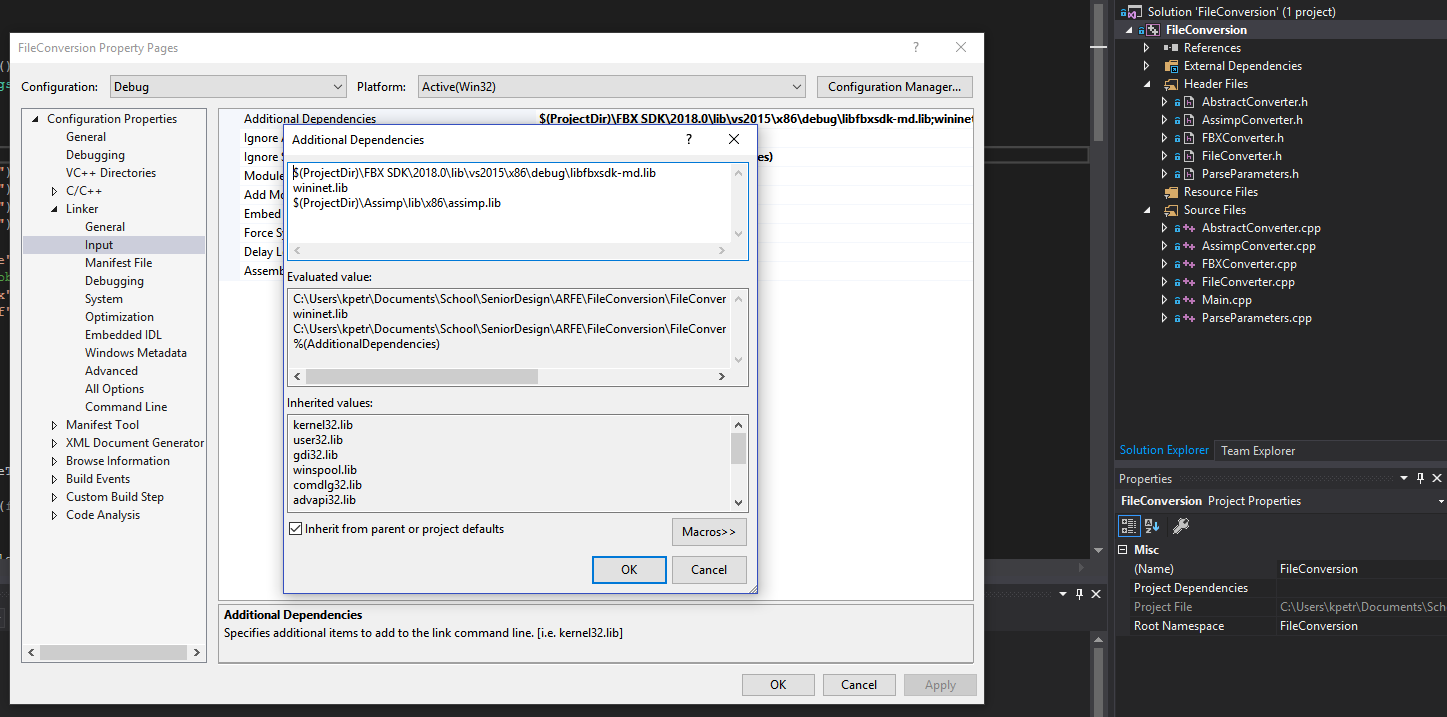
\includegraphics[width=\textwidth]{Deployment/fileConversionVSConfig_Linker_Input}
                \centering
                \caption{File Conversion VS Configuration Linker Configuration - Input}
                \label{fig:fileconversionVSConfig2}
            \end{figure}
    \end{enumerate}

    \subsection{Distribution}

        Two items are needed when distributing the file conversion software: the executable (\texttt{FileConversion.exe}) and a DLL (\texttt{assimp-vc140-mt.dll}).  The DLL is needed for the assimp library for file conversions.

        \subsubsection{Location in the Website}
        The \texttt{FileConversion.exe} along with it's associated (\texttt{assimp-vc140-mt.dll} are located in the ``UploadedFiles" folder under the root web directory (``~/UploadedFiles'').  This directory serves as the root directory for temporary intermediate file storage between the users and Azure Blob Storage.